\subsection{Implementierung in C\#\hfill\textnormal{\emph{Walter}}}
Die Software wurde mithilfe von C\# implementiert, aus dem Hintergrund, dass Unity diese Sprache verwendet. So kann das ganze Projekt in einer Sprache einheitlich implementiert werden.  

C\# eignet sich durch die Objekt-Orientierung sehr gut für die Beschreibung komplexer Systeme. Jedes Objekt, welches in dem behandelten Szenario vorhanden ist, wurde im Code implementiert. Die vorhandenen Klassen werden in einem Klassen-Diagramm in Abbildung \ref{ClassDiagram} gezeigt.

Jede dieser Klassen hat verschiedene Methoden und Attribute. Die Objekte werden in Abschnitt \ref{obj} weiter erläutert. 

\subsubsection{Objekte}
\label{obj}
Die Simulation des Roboters, sollte so genau wie möglich sein, daher wurden alle Gegenstände, die mit dem Roboter interagieren als eigenständige Objekte angelegt. Bei den Objekten kann es sich, zum Beispiel, um sogenannte Ground-Objekte handeln. Diese Ground-Objekte beschreiben jedes Objekt, welches auf der Karte zu finden ist. So erben die Obstacle-Objekte von den Ground-Objekten selbige Position und das traversable Attribut. Dies wird in Abbildung \ref{erben} verdeutlicht. 

\begin{figure}[H]
  \centering{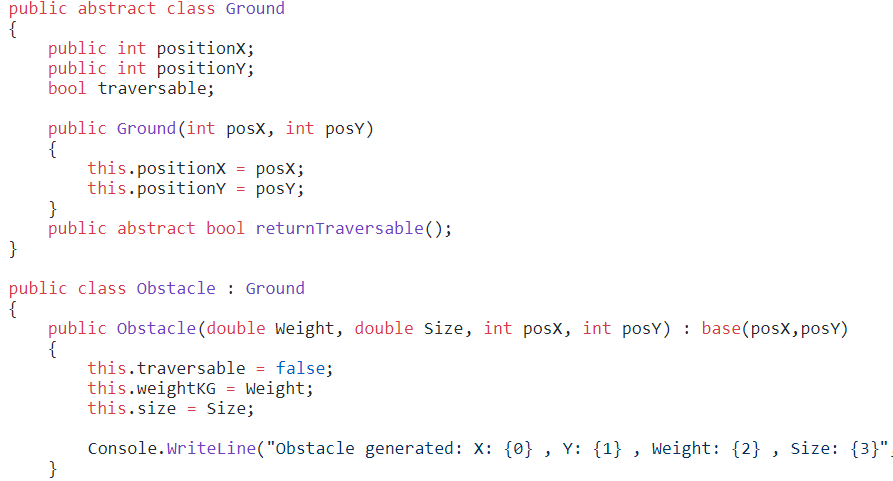
\includegraphics[width=1.0\linewidth]{Abbildungen/implementierung/vererbung.PNG}}
  \caption{Vererbung von Ground-Objekt zu Obstacle-Objekt}
  \label{erben}
\end{figure}
Zusätzlich zu den Ground-Objekten gibt es, Peripherie-Geräte für den Roboter, wie zum Beispiel Kamera oder Mikrophon. Auch Bauteile wie Motoren wurde mit verschiedenen Eigenschaften implementiert. So kann ein Motor einen Namen, Anfangs- und End-position, Geschwindigkeit und State besitzen.

Die Rescue Bot Klasse, die in Abbildung \ref{bot2} zu sehen ist, beinhaltet die Sensoren und Aktoren, welche durch den Roboter miteinander interagieren. Dazu zählen Kamera, Antennen, der LIDAR Sensor und Greifarm.

\begin{figure}[H]
  \centering{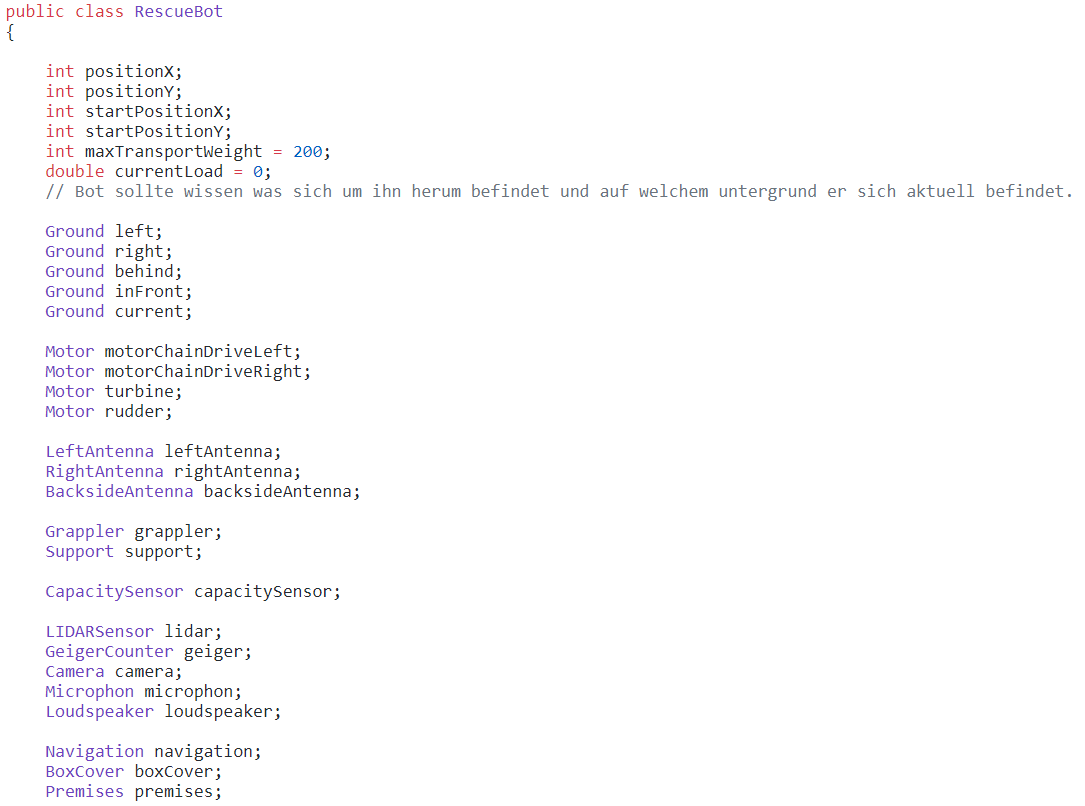
\includegraphics[width=1.0\linewidth]{Abbildungen/implementierung/rescueBotClass2.PNG}}
  \caption{Rescue Bot Klasse}
  \label{bot2}
\end{figure}
So befindet sich zum Beispiel der LIDAR Sensor, der Greifarm und der Geigerzähler innerhalb der Rescue Bot Klasse. Durch diese Verkettung kann der Rescue Bot auf die Methoden der Geräte, ebenfalls Klassen, zugreifen. 


\subsubsection{Karte}
\label{map_}
Die Karte wird aus einem zweidimensionalen Array generiert. Dieses Eingabe Array besteht dabei aus verschieden Strings. Aus dem Input wird mithilfe einer Switch-Case Anweisung ein neues Array generiert, welches aus Objekten besteht, die den Strings innerhalb des Eingabe Arrays entsprechen. Das Eingabe Array wird in Abbildung \ref{map} dargestellt. 

\begin{figure}[H]
  \centering{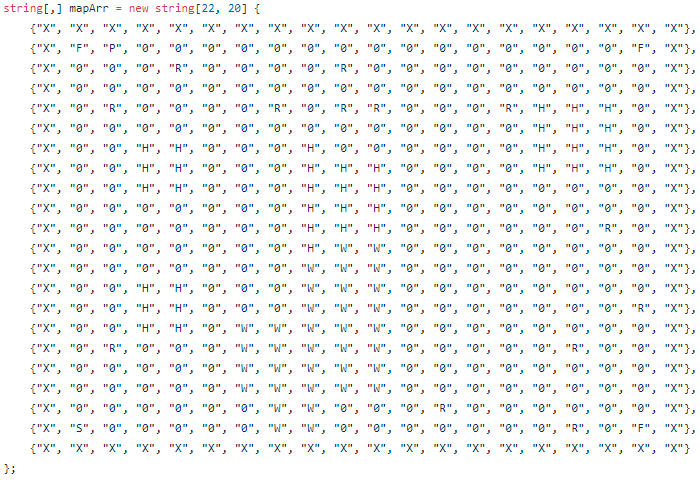
\includegraphics[width=1.0\linewidth]{Abbildungen/implementierung/mapArr.PNG}}
  \caption{Zweidiemensionales Array als Karte}
  \label{map}
\end{figure}

So wird zum Beispiel aus einem "R“ innerhalb des Eingabe Arrays ein radioaktives Objekt erstellt, mit zufälliger Größe, Gewicht und Strahlung als Attribute. Der Prozess der Objekt-Instanziierung wird in Abbildung \ref{rad} veranschaulicht. 

Eine Aufschlüsselung der einzelnen Buchstaben und ihre Bedeutung wird in folgender Tabelle erläutert:
\begin{table}[H]
\centering
\begin{tabular}{l|l}
Zeichen & Bedeutung                 \\ 
\hline
0       & Frei befahrbarer Untergrund             \\
W       & Wasser                    \\
X       & Wand / Äußere Begrenzung  \\
S       & Startpunkt                \\
F       & Funkturm                  \\
R       & Radioaktives Objekt       \\
P       & Zielperson  
\label{buchstaben}
\end{tabular}
\end{table}

Die Objekte werden direkt in das objArr Array gespeichert, was beispielhaft in der vorletzten Zeile in Abbildung \ref{map} zu sehen ist. 


\begin{figure}[H]
  \centering{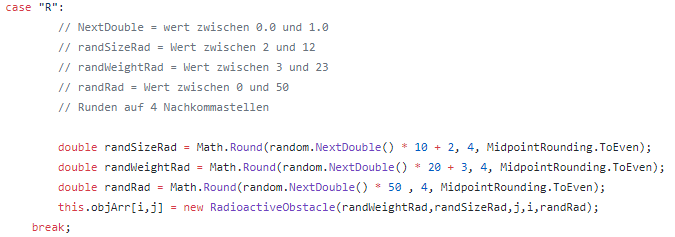
\includegraphics[width=1.0\linewidth]{Abbildungen/implementierung/createRadObj.PNG}}
  \caption{Instanziierung von Radioaktiven Objekten}
  \label{rad}
\end{figure}

\subsubsection{Erkennung und Bergen von Radioaktiven Gegenständen}
\label{erk}
Die Erkennung und das Bergen von radioaktiven Gegenständen ist eines der Hauptfeatures des Rescue Bots. Die Erkennung dieser Objekte erfolgt in mehreren Schritten. Bevor der Bot sich in Bewegung versetzt, wird über den LIDAR Sensor die unmittelbare Umgebung gescannt. Hierbei werden die Punkte vor, hinter, links, rechts und unter dem Bot erkannt. Felder, welche diagonal zum Bot liegen, werden ignoriert. Sollte sich auf einem Feld, das direkt an den Bot grenzt ein radioaktives Objekt liegen, wird dieses aufgesammelt, wenn es folgenden Kriterien entspricht: Größe, abgegebene radioaktive Strahlung und Gewicht. Der maximale Wert in allen drei Fällen beträgt 100 Einheiten.

Zuerst wird die Größe des Objektes mithilfe das LIDAR Sensors geprüft. Liegt das Objekt unterhalb der maximalen Größe, wird der Greifer in Richtung des Objektes bewegt und die radioaktive Strahlung durch den Geigerzähler gemessen. Sollte die Strahlung den bestimmten Wert übersteigen, wird das Objekt gegriffen und das Gewicht gemessen. Ist auch das Gewicht geringer als das maximale, kann der Gegenstand eingesammelt werden. 

Dieser Prozess kann auch anhand des Aktivitätsdiagramms in Abbildung \ref{Rescue_object} nachvollzogen werden. 
\subsubsection{Navigation}
\label{nav}
Ziel ist es, den Bot autonom durch die generierte Karte fahren zu lassen. Um dies zu realisieren, beinhaltet die Karte drei Funktürme.

Jeder dieser Funktürme besitzt eine ID und Position auf der Karte. Diese Daten kann jeder der drei Funktürme an den Rescue Bot senden. Aus entsprechenden Daten kann der Bot entscheiden welcher Funkturm der nächste ist und in selbige Richtung fahren. 

Die Berechnung der Distanz wird in Abbildung \ref{dist} gezeigt. 
\begin{figure}[H]
  \centering{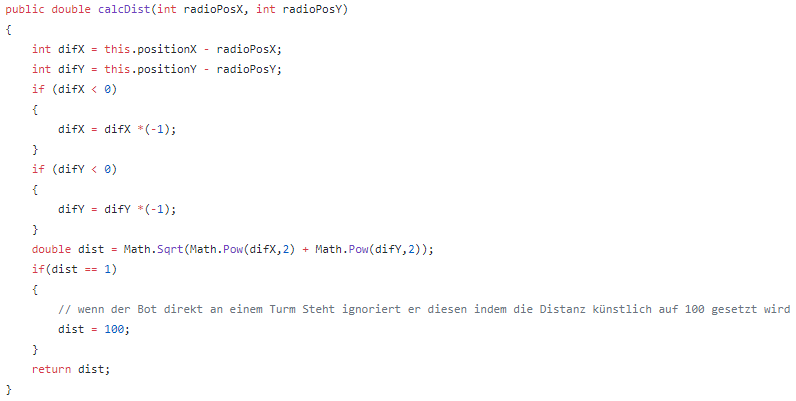
\includegraphics[width=1.0\linewidth]{Abbildungen/implementierung/calcDist.PNG}}
  \caption{Berechnung der Distanz zwischen zwei Punkten auf einer Fläche durch den Satz des Pythagoras}
  \label{dist}
\end{figure}

Entspricht die gemessene Distanz einer Längeneinheit (dist = 1), steht der Bot direkt neben dem Funkturm. Um den Funkturm für weitere Berechnungen zu ignorieren, wird die Distanz auf eine hohe Zahl gesetzt, in Abbildung \ref{dist} ist dies im Beispiel 100. Das hat die Folge, dass nun die kürzeste Distanz zwischen den zwei verbleibenden Funktürmen gewählt wird.

Um sich zu den verschiedenen Funktürmen zu bewegen, können unterschiedliche Ansätze gewählt werden. Im Folgenden wird einer dieser Ansätze beschrieben.

In diesem Ansatz wird die Differenz der X- und Y-Koordinate berechnet und anschließend versucht diesen Differenzwert gegen Null zu bringen. Dies geschieht indem zwischen einer Bewegung in X-Richtung und in Y-Richtung gewechselt wird, um eine diagonale Bewegung zu ermöglichen. Auf diese Art und Weise kann die gefahrene Strecke minimiert werden. 

Sollten sich Hindernisse auf dem Weg befinden, weicht der Bot in eine zufällige Richtung aus und versucht erneut den Weg zum Ziel einzuschlagen. Dieser Vorgang wird so lange wiederholt, bis das Hindernis umfahren ist.  

\subsubsection{Test Case}
\label{test}
Zum Testen des Systems wurde ein Szenario entwickelt, welches einige der Funktionen des Roboters überprüft. 

So soll getestet werden ob der Roboter den Rotor einschaltet, wenn er schwimmt, ob er radioaktive Gegenstände eigenständig findet und einsammelt, und zum Schluss, ob eine Zielperson erkannt wird und mit ihr interagiert werden kann. 

Folgende Einschränkungen wurden dabei festgelegt: 

\begin{itemize}
	\item Es gibt genau eine Zielperson, welche sich an einem der in Abschnitt \ref{nav} beschriebenen Funktürme befinden muss
	\item Die Radioaktiven Gegenstände dürfen frei verteilt werden
	\item Hindernisse dürfen frei verteilt werden
	\item Es wird auf Sichteinschränkungen durch Nebel verzichtet
	\item Bewegliche Hindernisse werden nicht berücksichtigt und entfernt
\end{itemize}
 
Das Ziel des Test-Case ist, den Roboter bis zum Erkennen einer Zielperson an den Funktürmen vorbeifahren zu lassen. Während dieser Suche, soll jedes radioaktive Objekt eingesammelt werden, solange der Bot nicht voll beladen ist. Zudem soll angezeigt werden, welcher Motor aktuell verwendet wird.

Der Programmablauf ist als erfolgreich anzusehen, wenn die Zielperson gefunden und die aktuelle radioaktive Ladung ausgegeben wurde.

\begin{figure}[H]
  \centering{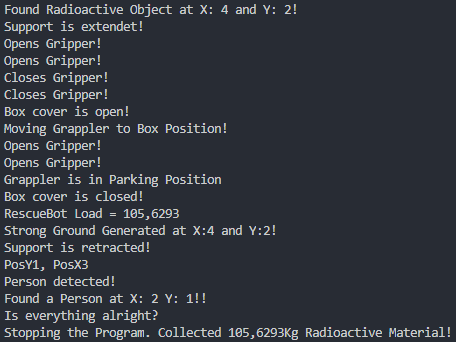
\includegraphics[width=1.0\linewidth]{Abbildungen/implementierung/output.PNG}}
  \caption{Ausgabe des Programms (Einsammeln von Radioaktiven Gegenständen und Interaktion mit Zielpersonen)}
  \label{output}
\end{figure}

\begin{figure}[H]
  \centering{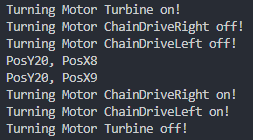
\includegraphics[width=1.0\linewidth]{Abbildungen/implementierung/waterr.PNG}}
  \caption{Ausgabe des Programms (Verwendung des Aktuellen Motors)}
  \label{waterr}
\end{figure}

Wie in Abbildung \ref{output} abgelesen werden kann, findet der Rescue-Bot ein radioaktives Objekt, fährt den Greifer aus und entfernt es. Im weiteren Programmverlauf findet der Rescue-Bot die Zielperson und hat begonnen mit ihr zu interagieren. Somit ist die Funktion des Einsammelns von radioaktiven Gegenständen und der Interaktion mit Personen funktionsfähig.  

In Abbildung \ref{waterr} wird dargestellt welche Motoren aktuell verwendet werden und welche inaktiv sind. Fährt der Rescue Bot auf der Wasseroberfläche, so ist die Turbine in Betrieb, fährt er auf Land, sind beide Motoren für den Kettenantrieb aktiviert. Somit konnte auch diese Funktion validiert werden.


